\documentclass[tikz]{standalone}
\usetikzlibrary{positioning, arrows.meta}
\begin{document}
    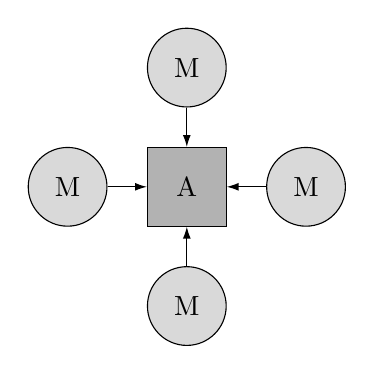
\begin{tikzpicture}[
        A/.style = {draw, black, fill=black!30, minimum height=1cm, minimum width=1cm, inner sep=2pt},
        M/.style = {draw, black, fill=black!15, circle, minimum size=1cm, inner sep=2pt},
        arrow/.style = {-{Latex[length=1.5mm, width=1.0mm]},align=flush center}
    ]
        \node[A] (A) {A};
        \node[M, left=0.5cm of A] (Ml) {M};
        \node[M, right=0.5cm of A] (Mr) {M};
        \node[M, below=0.5cm of A] (Mb) {M};
        \node[M, above=0.5cm of A] (Ma) {M};
        \draw[arrow] (Ml) -> (A);
        \draw[arrow] (Mr) -> (A);
        \draw[arrow] (Mb) -> (A);
        \draw[arrow] (Ma) -> (A);
    \end{tikzpicture}
\end{document}
